
\chapter{GCSE Revision - Angles (and Bearings)}

\begin{enumerate}
  \item \mrk{4}
  \begin{figure}[H]
    \centering
    \begin{tikzpicture}[scale=1.3]
      \tkzDefPoints{-4/0/P,1/0/Q,0/2/T,3/0/R,5/1.8/L}
      \tkzDrawPolygon(P,Q,T)
      \tkzDrawSegments(Q,R)
      \tkzMarkAngle[size=0.6, mark=none](R,Q,T)
      \tkzMarkAngle[size=1, mark=none](Q,P,T)
      \tkzMarkSegments[mark=|](P,Q P,T)

      \tkzLabelAngle[pos=0.3](R,Q,T){\small $\ang{110}$}
      \tkzLabelAngle[pos=0.7](Q,P,T){\small $y^\circ$}
      \tkzLabelPoints[below](P,Q,R)
      \tkzLabelPoint[above](T){T}
      \tkzLabelPoint[above](L){Diagram \textbf{NOT}}
      \tkzLabelPoint[below](L){accurately drawn}
    \end{tikzpicture}
  \end{figure}
  $PQR$ is a straight line. $PT = PQ$.
  \begin{enumerate}
    \item Work out the value of $y$.\strch\\\vspace*{0cm}\hfill\dline
    \item Give reasons for your answer.\\
    \hdashrule{0.85\textwidth}{1pt}{1ex}\\
    \hdashrule{0.85\textwidth}{1pt}{1ex}\strch
  \end{enumerate}

  \newpage
  \item \mrk{4}
  \begin{figure}[H]
    \centering
    \begin{tikzpicture}
      \tkzDefPoints{0/0/A, 3/0/B, 7/3/L}
      \tkzDefRegPolygon[side,sides=5,name=P](A,B)
      \tkzDrawPolygon[thick](P1,P...,P5)
      \tkzLabelPoint[above](L){Diagram \textbf{NOT}}
      \tkzLabelPoint[below](L){accurately drawn}
    \end{tikzpicture}
  \end{figure}
  Work out the size of an exterior angle of a regular pentagon.\strch\\\vspace*{0cm}\hfill\dline
  \item \mrk{3}
  \begin{figure}[H]
    \centering
    \begin{tikzpicture}
      \tkzDefPoints{0/0/C, 2/0/M, 6/0/D, 0/3/A, 6/3/B, 4/5/L, 9/5/P}
      \tkzInterLL(A,B)(M,L)
      \tkzGetPoint{N}
      \tkzDrawSegments[->, >=latex, thick](A,B C,D)
      \tkzDrawSegments[thick](M,L)
      \tkzMarkAngle[size=0.5, mark=none](L,N,A)
      \tkzMarkAngle[size=1, mark=none](D,M,L)

      \tkzLabelAngle[pos=0.3](L,N,A){\small $y$}
      \tkzLabelAngle[pos=0.7](D,M,L){\small $\ang{60}$}

      \tkzLabelPoint[left](A){$A$}
      \tkzLabelPoint[left](C){$C$}
      \tkzLabelPoint[right](B){$B$}
      \tkzLabelPoint[right](D){$D$}
      \tkzLabelPoint[below right](M){$M$}
      \tkzLabelPoint[below right](N){$N$}
      \tkzLabelPoint[above right](L){$L$}

      \tkzLabelPoint[above](P){Diagram \textbf{NOT}}
      \tkzLabelPoint[below](P){accurately drawn}
    \end{tikzpicture}
  \end{figure}
  $ANB$ is parallel to $CMD$. $LNM$ is a straight line. Angle $LMD = \ang{68}$.
  \begin{enumerate}
    \item Work out the size of the angle marked $y$.\strch\\\vspace*{0cm}\hfill\dline$^\circ$
    \item Give reasons for your answer.\\
    \hdashrule{0.85\textwidth}{1pt}{1ex}\\
    \hdashrule{0.85\textwidth}{1pt}{1ex}\strch
  \end{enumerate}

  \newpage
  \item \mrk{2}
  \begin{figure}[H]
    \centering
    \begin{tikzpicture}
      \tkzDefPoints{0/0/D, 1/-1/P, 7/0/C, 0/2/A, 7/2/B, 5.5/3.25/S, 9.5/3.25/L}
      \tkzInterLL(A,B)(P,S)
      \tkzGetPoint{R}
      \tkzInterLL(D,C)(P,S)
      \tkzGetPoint{Q}
      \tkzDrawSegments[->, >=latex, thick](A,B D,C)
      \tkzDrawSegments[thick](P,S)
      \tkzMarkAngle[size=0.7, mark=none](S,R,A)
      \tkzMarkAngle[size=1.2, mark=none](B,R,S)
      \tkzMarkAngle[size=1, mark=none](C,Q,R)

      \tkzLabelAngle[pos=0.3](S,R,A){\small $\ang{125}$}
      \tkzLabelAngle[pos=0.8](B,R,S){\small $\ang{55}$}
      \tkzLabelAngle[pos=0.7](C,Q,R){\small $x$}

      \tkzLabelPoint[left](A){$A$}
      \tkzLabelPoint[right](C){$C$}
      \tkzLabelPoint[right](B){$B$}
      \tkzLabelPoint[left](D){$D$}
      \tkzLabelPoint[below left](P){$P$}
      \tkzLabelPoint[below right](Q){$Q$}
      \tkzLabelPoint[below right](R){$R$}
      \tkzLabelPoint[above right](S){$S$}

      \tkzLabelPoint[above](L){Diagram \textbf{NOT}}
      \tkzLabelPoint[below](L){accurately drawn}
    \end{tikzpicture}
  \end{figure}
  $ARB$ is parallel to $DQC$. $PQRS$ is a straight line. Angle $SRB = \ang{55}$.
  \begin{enumerate}
    \item Find the size of the angle marked $x$.\strch\\\vspace*{0cm}\hfill\dline$^\circ$
    \item Give a reason for your answer.\\
    \hdashrule{0.85\textwidth}{1pt}{1ex}\strch
  \end{enumerate}
  \item \mrk{3}
  \begin{figure}[H]
    \centering
    \begin{tikzpicture}[scale=0.7]
      \tkzDefPoints{0/0/A, 6/0/C, 6/4/B, 9/4/L}
      \tkzDrawPolygon(A,B,C)
      \tkzDefLine[perpendicular=through C](A,B)
      \tkzGetPoint{F}
      \tkzInterLL(A,B)(F,C)
      \tkzGetPoint{P}
      \tkzDrawSegment(C,P)

      \tkzMarkRightAngle(A,P,C)
      \tkzMarkRightAngle(A,C,B)

      \tkzLabelPoint[below left](A){$A$}
      \tkzLabelPoint[below](C){$C$}
      \tkzLabelPoint[above](B){$B$}
      \tkzLabelPoint[above](P){$P$}

      \tkzLabelPoint[above](L){Diagram \textbf{NOT}}
      \tkzLabelPoint[below](L){accurately drawn}
    \end{tikzpicture}
  \end{figure}
  In the diagram, $ABC$ is a triangle, angle $ACB = \ang{90}$, $P$ lies on the line $AB$, $CP$ is perpendicular to $AB$.\\
  Prove that the angles of triangle $APC$ are the same as the angles of triangle $CPB$.\strch

  \newpage
  \item \mrk{4}
  \begin{figure}[H]
    \centering
    \begin{tikzpicture}
      \tkzDefPoints{0/0/A, 2/0/B, 7/3/L}
      \tkzDefRegPolygon[side,sides=6,name=P](A,B)
      \tkzDrawPolygon[thick](P1,P...,P6)

      \tkzDefSquare(P4,P3)
      \tkzGetPoints{E}{F}
      \tkzDrawPolygon[thick](P3,P4,F,E)

      \tkzMarkAngle[size=0.7, mark=none](F,P4,P5)
      \tkzLabelAngle[pos=0.3](F,P4,P5){$a$}

      \tkzLabelPoint[above](L){Diagram \textbf{NOT}}
      \tkzLabelPoint[below](L){accurately drawn}
    \end{tikzpicture}
  \end{figure}
  The diagram shows a regular hexagon and a square. Calculate the size of the angle $a$.\strch\\
  \vspace*{0cm}\hfill\dline$^\circ$
  \item \mrk{3}
  \begin{figure}[H]
    \centering
    \begin{tikzpicture}
      \tkzDefPoints{0/0/A,4/0/B,6/3/C,9/0/E, 11/3/L}
      \tkzDefParallelogram(A,B,C)
      \tkzGetPoint{D}
      \tkzDrawPolygon(A,B,C,D)
      \tkzDrawPolygon(B,C,E)
      \tkzDrawSegment(A,C)

      \tkzMarkAngle[size=1.5, mark=none](C,E,B)
      \tkzLabelAngle[pos=1](C,E,B){$\ang{48}$}

      \tkzMarkSegments[mark=|](A,D A,B B,C D,C B,E)

      \tkzLabelPoints(A,B,E)
      \tkzLabelPoints[above right](C,D)

      \tkzLabelPoint[above](L){Diagram \textbf{NOT}}
      \tkzLabelPoint[below](L){accurately drawn}
    \end{tikzpicture}
  \end{figure}
  $ABCD$ is a rhombus. $BCE$ is an isosceles triangle. $ABE$ is a straight line.\\
  Work out the size of angle $DCA$.\strch\\\vspace*{0cm}\hfill\dline$^\circ$

  \newpage
  \item \mrk{7}
  \begin{figure}[H]
    \centering
    \begin{tikzpicture}
      \tkzDefPoints{0/0/A, 6/0/B, 9/0/C, 2/3/P, 11/3/L}
      \tkzDrawSegments(A,B B,C)
      \tkzDrawPolygon(A,B,P)

      \tkzMarkAngle[size=1.2, mark=none](A,P,B)
      \tkzMarkAngle[size=1.8, mark=none](B,A,P)
      \tkzMarkAngle[size=0.55, mark=none](C,B,P)

      \tkzLabelAngle[pos=0.8](A,P,B){\small $x+50$}
      \tkzLabelAngle[pos=1.2](B,A,P){\small $2x-10$}
      \tkzLabelAngle[pos=0.3](C,B,P){\small $y$}

      \tkzLabelPoints[below](A,B,C)
      \tkzLabelPoint[above](P){$P$}

      \tkzLabelPoint[above](L){Diagram \textbf{NOT}}
      \tkzLabelPoint[below](L){accurately drawn}
    \end{tikzpicture}
  \end{figure}
  All angles are measured in degrees. $ABC$ is a straight line.\\
  Angle $APB = x + 50$, Angle $PAB = x - 10$, Angle $PBC = y$.
  \begin{enumerate}
    \item Show that y = 3x + 40. Give reasons for each stage of your working.\mrk{3}\strch
    \item Given that $y = 145$\mrk{4}
    \begin{enumerate}
      \item work out the value of $x$.\strch\\\vspace*{0cm}\hfill$x=$\dline
      \item work out the size of the largest angle in triangle $ABP$.\strch\\\vspace*{0cm}\hfill\dline$^\circ$
    \end{enumerate}
  \end{enumerate}

  \newpage
  \item \mrk{3}
  \begin{figure}[H]
    \centering
    \begin{tikzpicture}
      \tkzDefPoints{0/0/A,5/0/B,6/3/C, 9/3/L}
      \tkzDefParallelogram(A,B,C)
      \tkzGetPoint{D}

      \tkzDefMidPoint(A,B)
      \tkzGetPoint{E}
      \tkzDefMidPoint(B,C)
      \tkzGetPoint{F}
      \tkzDefMidPoint(D,C)
      \tkzGetPoint{G}
      \tkzDefMidPoint(A,D)
      \tkzGetPoint{H}

      \tkzDrawSegments[->](A,E B,F D,G A,H)

      \tkzMarkAngles[size=0.7, mark=none](B,A,D D,C,B)
      \tkzMarkAngles[size=1.3, mark=none](A,D,C C,B,A)

      \tkzLabelAngle[pos=0.4](B,A,D){\small $2x$}
      \tkzLabelAngle[pos=0.4](D,C,B){\small $2x$}

      \tkzLabelAngle[pos=0.75](A,D,C){\small $3x-15$}
      \tkzLabelAngle[pos=0.75](C,B,A){\small $2x+24$}

      \tkzDrawPolygon(A,B,C,D)
      \tkzLabelPoints(A,B)
      \tkzLabelPoints[above right](C,D)

      \tkzLabelPoint[above](L){Diagram \textbf{NOT}}
      \tkzLabelPoint[below](L){accurately drawn}
    \end{tikzpicture}
  \end{figure}
  The diagram shows a parallelogram.\\
  The sizes of the angles, in degrees, are as pictured. Work out the value of $x$.\strch\\
  \vspace*{0cm}\hfill$x=$\dline
  \item \mrk{4}
  \begin{figure}[H]
    \centering
    \begin{tikzpicture}
      \tkzDefPoints{0/0/A, 2/0/B, 5/0/L}
      \tkzDefRegPolygon[center,sides=8,name=P](A,B)
      \tkzDrawPolygon[thick](P1,P...,P8)

      \tkzDefRegPolygon[side,sides=6,name=Q](P5,P4)
      \tkzDrawPolygon[thick](Q1,Q...,Q6)

      \tkzMarkAngles[size=0.7, mark=none](Q6,P5,P6)
      \tkzLabelAngle[pos=0.4](Q6,P5,P6){\small $x$}

      \tkzLabelPoint[above](L){Diagram \textbf{NOT}}
      \tkzLabelPoint[below](L){accurately drawn}
    \end{tikzpicture}
  \end{figure}
  The diagram shows a regular hexagon and a regular octagon.\par
  Calculate the size of the angle marked $x$.\\
  You must show all your working.\strch\\\vspace*{0cm}\hfill\dline$^\circ$
  
  \newpage
  \item The diagram shows the position of a lighthouse $L$ and a harbour $H$.\mrk{4}
  \begin{figure}[H]
    \centering
    \begin{tikzpicture}
      \tkzDefPoints{2/2/L, 7/0/H, 2/5/N1, 7/3/N2, 10/3/P}
      \tkzDrawSegment(L,H)
      \tkzDrawSegments[->, -Triangle](L,N1 H,N2)
      \tkzDrawPoints[shape=cross out,size=4, thick](H,L)

      \tkzLabelPoints[below](L,H)
      \tkzLabelPoint[above](N1){$\vb{N}$}
      \tkzLabelPoint[above](N2){$\vb{N}$}

      \tkzLabelPoint[above](P){Diagram \textbf{NOT}}
      \tkzLabelPoint[below](P){accurately drawn}
    \end{tikzpicture}
  \end{figure}
  The scale of the diagram is $1$ cm represents $5$ km
  \begin{enumerate}
    \item Work out the real distance between $L$ and $H$.\strch\\\vspace*{0cm}\hfill\dline km
    \item Measure the bearing of $H$ from $L$.\strch\\\vspace*{0cm}\hfill\dline$^\circ$
    \suspend{enumerate}
    A boat $B$ is $20$ km from $H$ on a bearing of $\ang{040}$
    \resume{enumerate}
    \item On the diagram, mark the position of boat $B$ with a cross ($\times$). Label it $B$.\strch
  \end{enumerate}
  \item \mrk{3}
  \begin{figure}[H]
    \centering
    \begin{tikzpicture}
      \tkzDefPoints{0/3/A, 7/3/C, 0/0/D, 7/0/F, 2/3/B, 6.5/-1.5/G, 10/3/L}
      \begin{scope}[decoration={
        markings,
        mark=at position 0.2 with {\arrow{>}}}
        ]
        \tkzDrawSegments[postaction={decorate}](A,C D,F)
      \end{scope}
      \tkzDrawSegment(B,G)

      \tkzInterLL(D,F)(B,G)
      \tkzGetPoint{E}

      \tkzMarkAngles[size=0.5, mark=none](A,B,G)
      \tkzLabelAngle[pos=0.3](A,B,G){\small $x$}

      \tkzMarkAngles[size=1, mark=none](G,E,F)
      \tkzLabelAngle[pos=0.7](G,E,F){\small $\ang{47}$}

      \tkzLabelPoints[left](A, D)
      \tkzLabelPoints[right](C, F)
      \tkzLabelPoints[above](B)
      \tkzLabelPoints[below](G)
      \tkzLabelPoints[below left](E)

      \tkzLabelPoint[above](L){Diagram \textbf{NOT}}
      \tkzLabelPoint[below](L){accurately drawn}
    \end{tikzpicture}
  \end{figure}
  $ABC$ and $DEF$ are parallel lines. $BEG$ is a straight line. Angle $GEF = \ang{47}$.\\
  Work out the size of the angle marked $x$.\\
  Give reasons for your answer.\strch\\\vspace*{0cm}\hfill\dline$^\circ$
  
  \newpage
  \item \mrk{3}
  \begin{figure}[H]
    \centering
    \begin{tikzpicture}[scale=0.7]
      \tkzDefPoints{-1/1/A, 3/4/B, 7/1/C, 1.5/2/D, 9/2/E, 2/5/F, 6/0/G, 15/4/L}
      \begin{scope}[decoration={
        markings,
        mark=at position 0.9 with {\arrow[thick]{Stealth}}}
        ]
        \tkzDrawLine[postaction={decorate}, add=0.4 and 0.3](A,B)
        \tkzDefLine[parallel=through C](A,B)
        \tkzGetPoint{c'}
        \tkzDrawLine[postaction={decorate}, add=0.4 and 0.3](C,c')
      \end{scope}
      \tkzDrawLines[add=0.4 and 0.2](D,E)
      \tkzDrawLines[add=0 and 0.2](F,G)

      \tkzInterLL(D,E)(C,c')
      \tkzGetPoint{m1}
      \tkzMarkAngles[size=1, mark=none](C,m1,E)
      \tkzLabelAngle[pos=0.6](C,m1,E){$\ang{150}$}

      \tkzInterLL(F,G)(C,c')
      \tkzGetPoint{m2}
      \tkzMarkAngles[size=1.2, mark=none](G,m2,C)
      \tkzLabelAngle[pos=0.7](G,m2,C){$\ang{85}$}

      \tkzInterLL(A,B)(F,G)
      \tkzGetPoint{m3}
      \tkzMarkAngles[size=1.2, mark=none](A,m3,G)
      \tkzLabelAngle[pos=0.7](A,m3,G){\Large $y^\circ$}

      \tkzInterLL(A,B)(D,E)
      \tkzGetPoint{m4}
      \tkzMarkAngles[size=1, mark=none](A,m4,D)
      \tkzLabelAngle[pos=0.6](A,m4,D){\Large $x^\circ$}

      \tkzLabelPoint[above](L){Diagram \textbf{NOT}}
      \tkzLabelPoint[below](L){accurately drawn}
    \end{tikzpicture}
  \end{figure}
  \begin{enumerate}
    \item Find the value of $x$.\mrk{1}\strch\\\vspace*{0cm}\hfill\dline
    \item Find the value of $y$. Give reasons for your answer.\mrk{2}\strch\\\vspace*{0cm}\hfill\dline
  \end{enumerate}
  \item The bearing of a ship from a lighthouse is $0\ang{050}$. Work out the bearing of the lighthouse from the ship.\mrk{2}\strch\\\vspace*{0cm}\hfill\dline$^\circ$
  
  \newpage
  \item The diagram shows part of a pattern made from tiles.\mrk{4}
  \begin{figure}[H]
    \centering
    \begin{tikzpicture}[scale=0.7]
      % \tkzInit[xmax=7,ymax=10]
      % \tkzGrid[sub,orange]

      \tkzDefPoints{2/7/A,5/7/B, 0.5/7.5/D, 6.5/7.5/E}

      \tkzDefTriangle[equilateral](B,A)
      \tkzGetPoint{C}
      \tkzDrawPolygon[fill=gray, opacity=0.6](A,B,C)

      \tkzDefShiftPoint[A](0,-7){A'}
      \tkzDefShiftPoint[B](0,-7){B'}

      \tkzDefTriangle[equilateral](A',B')
      \tkzGetPoint{C'}
      \tkzDrawPolygon[fill=gray, opacity=0.6](A',B',C')

      \tkzDefShiftPoint[D](0,-8){D'}
      \tkzDefShiftPoint[E](0,-8){E'}

      \tkzDefShiftPoint[D](-0.5,1.5){F}
      \tkzDefShiftPoint[E](0.5,1.5){G}

      \tkzDefShiftPoint[D'](-0.5,-1.5){F'}
      \tkzDefShiftPoint[E'](0.5,-1.5){G'}

      \tkzDefShiftPoint[C](0,1.8){T1}
      \tkzLabelPoint[above](T1){\textbf{Tile B}}

      \tkzDefShiftPoint[C'](0,-1.8){T2}
      \tkzLabelPoint[below](T2){\textbf{Tile B}}

      \tkzDefShiftPoint[C](0,3){t1}
      \tkzLabelPoint[above](t1){\textbf{Tile A}}

      \tkzDefShiftPoint[C'](0,-3){t2}
      \tkzLabelPoint[below](t2){\textbf{Tile A}}

      \tkzLabelPoint[above left](C'){\textbf{Tile A}}
      \tkzLabelPoint[above right](C'){\textbf{Tile A}}

      \tkzDefShiftPoint[G](2.5,-1){L}

      \tkzDrawSegments(A,D B,E A',D' B',E' D,F E,G D',F' E',G' C,C')

      \tkzLabelPoint[above](L){Diagram \textbf{NOT}}
      \tkzLabelPoint[below](L){accurately drawn}
    \end{tikzpicture}
  \end{figure}
  The pattern is made from two types of tiles, tile A and tile B.\\
  Both tile A and tile B are regular polygons. Work out the number of sides tile A has.\strch\\\vspace*{0cm}\hfill\dline
  \item \mrk{4}
  \begin{figure}[H]
    \centering
    \begin{tikzpicture}
      \tkzDefPoints{0/0/D,6/0/C,7/4/B,2.2/2/F,10/3.5/L}
      \tkzDefParallelogram(D,C,B)
      \tkzGetPoint{A}

      \begin{scope}[decoration={
        markings,
        mark=at position 0.4 with {\arrow[thick]{>>}}}
        ]
        \tkzDrawSegment[postaction={decorate}](A,B)
        \tkzDrawSegment[postaction={decorate}](D,C)
      \end{scope}

      \begin{scope}[decoration={
        markings,
        mark=at position 0.7 with {\arrow[thick]{>}}}
        ]
        \tkzDrawSegment[postaction={decorate}](D,A)
        \tkzDrawSegment[postaction={decorate}](C,B)
      \end{scope}

      \tkzInterLL(D,B)(F,C)
      \tkzGetPoint{E}

      \tkzDrawSegment(C,E)
      \tkzDrawSegment(D,B)

      \tkzMarkAngles[size=1.2, mark=none](D,A,B)
      \tkzLabelAngle[pos=0.7](D,A,B){\small $\ang{120}$}

      \tkzMarkAngles[size=1.5, mark=none](B,D,A)
      \tkzLabelAngle[pos=0.8](B,D,A){\small $\ang{38}$}

      \tkzMarkAngles[size=1.2, mark=none](C,E,B)
      \tkzLabelAngle[pos=0.7](C,E,B){\small $\ang{41}$}

      \tkzMarkAngles[size=2, mark=none](E,C,D)
      \tkzLabelAngle[pos=1.2](E,C,D){\Large $x$}

      \tkzLabelPoints[above](A,B)
      \tkzLabelPoints[below](C,D)
      \tkzLabelPoints[above left](E)

      \tkzLabelPoint[above](L){Diagram \textbf{NOT}}
      \tkzLabelPoint[below](L){accurately drawn}
      \end{tikzpicture}
  \end{figure}
  $ABCD$ is a parallelogram. Angle $ADB = \ang{38}$. Angle $BEC = \ang{41}$.
  Angle $DAB = \ang{120}$. Calculate the size of angle $x$. You must give reasons for your answer.\strch

  \newpage
  \item Here is a map. The position of a ship, $S$, is marked on the map.\mrk{3}
  \begin{figure}[H]
    \centering
    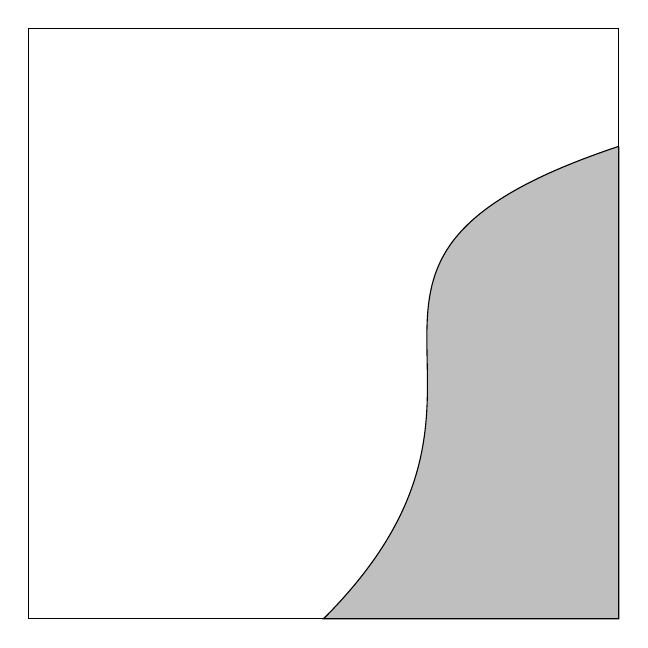
\begin{tikzpicture}[scale=1.5]
      \tkzDefPoints{1/1/S, 1/2.5/N, 3.36/2.5/C, 10/3.5/L}
      \draw (0,0) -- (5,0) -- (5,5) -- (0,5) -- (0,0); 
      \filldraw[fill=gray!50] (5,4) .. controls (2,3) and (4.5, 2) .. (2.5,0) -- (5,0) -- (5,4);
      \tkzDrawPoint[shape=cross out,thick](S)
      \tkzDrawPoint[shape=cross out,thick](C)
      \tkzDrawSegment[-stealth, thick](S,N)

      \tkzLabelPoints[below](S)
      \tkzLabelPoints[above](N)
      \tkzLabelPoints[right](C)
    \end{tikzpicture}
  \end{figure}
  Scale	1 cm represents 100 m.\\
  Point $C$ is on the coast. Ships must not sail closer than $500$ m to point $C$.\\
  The ship sails on a bearing of 0\ang{37}\\
  Will the ship sail closer than 500 m to point $C$?\\
  You must explain your answer.\strch




  




\end{enumerate}